\documentclass[11pt,a4paper]{article}
\usepackage[left=2.5cm,right=2cm, bottom=2cm]{geometry}
\usepackage[utf8]{inputenc}
\usepackage{amsmath}
\usepackage{amsfonts}
\usepackage{amssymb}
\usepackage{amsfonts}
\usepackage{amsmath}
\usepackage{graphicx}
\usepackage{subfigure}
\usepackage{color}
\usepackage{abstract}
\usepackage{float}
\usepackage[toc,page]{appendix}
\usepackage{hyperref}
\usepackage{fancyhdr}
\usepackage{algorithm} 
\usepackage{algpseudocode} 
\usepackage{listings}
\usepackage{xcolor} % for setting colors
% set the default code style
\lstset{
	frame=tb, % draw a frame at the top and bottom of the code block
	tabsize=4, % tab space width
	showstringspaces=false, % don't mark spaces in strings
	numbers=left, % display line numbers on the left
	commentstyle=\color{green}, % comment color
	keywordstyle=\color{blue}, % keyword color
	stringstyle=\color{red} % string color
}

\pagestyle{fancy}
\fancyhf{}
\rhead{\today}
\lhead{\bfseries Alexander Leitner 01525882}
\rfoot{}



\begin{document}
\begin{center}
	\fontsize{24pt}{10pt}\selectfont
	\textsc{\textbf{Computational Science on Many-Core Architectures  Exercise 8}}
\end{center}
\section*{Example 1 Libraries (5 Points)}
\subsection*{1) BoostCompute}
Part of the important calculation from the main() part.

\begin{lstlisting}[language=C++, caption={BoostCompute}]
	std::vector<ScalarType> x(N,1);
	std::vector<ScalarType> y(N,2);
	std::vector<ScalarType> init(N,0);
	
	compute::vector<ScalarType> d_x(x.size(), context);
	compute::vector<ScalarType> d_y(y.size(), context);
	compute::vector<ScalarType> d_xply(y.size(), context);
	compute::vector<ScalarType> d_xmiy(y.size(), context);
	
	// transfer data from the host to the device
	compute::copy(
	x.begin(), x.end(), d_x.begin(), queue
	);
	compute::copy(
	y.begin(), y.end(), d_y.begin(), queue
	);
	compute::copy(
	init.begin(), init.end(), d_xply.begin(), queue
	);
	compute::copy(
	init.begin(), init.end(), d_xmiy.begin(), queue
	);
	compute::transform(d_x.begin(), d_x.end(), 
	d_y.begin(), d_xply.begin(), compute::plus<ScalarType>{}, queue
	);
	compute::transform(d_x.begin(), d_x.end(), 
	d_y.begin(), d_xmiy.begin(), compute::minus<ScalarType>{}, queue
	);
	timer.reset();
	for (int i = 0; i < anz; i++)
	{
		dot = compute::inner_product(d_xply.begin(), d_xply.end(), 
		d_xmiy.begin(), 0.0, queue);
	}
	Boost_Time = timer.get()/anz;
	std::cout << "dot-prod_Boost: " << dot << std::endl;
\end{lstlisting}
\newpage
\subsection*{2) Thrust}
\begin{lstlisting}[language=C++, caption={Thrust}]
std::vector<ScalarType> x(N,1);
std::vector<ScalarType> y(N,2);
std::vector<ScalarType> v1pv2(N,0);
std::vector<ScalarType> v1mv2(N,0);

for (int i = 0; i < N; i++)
{
	v1pv2[i] = x[i] + y[i];
	v1mv2[i] = x[i] - y[i];
}
timer.reset();
for (int i = 0; i < anz; i++)
{
	thrust::host_vector<ScalarType> h_v1 = v1pv2;
	thrust::host_vector<ScalarType> h_v2 = v1mv2;
	
	thrust::device_vector<ScalarType> d_v1 = h_v1;
	thrust::device_vector<ScalarType> d_v2 = h_v2;
	
	dot = thrust::inner_product(d_v1.begin(), d_v1.end(),
	 d_v2.begin(), start);
}
VexCL_Time = timer.get()/anz;
std::cout << "dot-prod_Thrust: " << dot << std::endl;
\end{lstlisting}
\subsection*{3) VexCL}
\begin{lstlisting}[language=C++, caption={VexCL}]
timer.reset();
vex::Reductor<double, vex::SUM> DOT(ctx);
for (int i = 0; i < anz; i++)
{
	dot = DOT((X+Y)*(X-Y));
}
VexCL_Time = timer.get()/anz;
std::cout << "dot-prod_VexCL: " << dot << std::endl;
\end{lstlisting}
\newpage
\subsection*{4) ViennaCL}
\begin{lstlisting}[language=C++, caption={ViennaCL}]
viennacl::vector<double> x_VIE = viennacl::scalar_vector<double>(N, 1.0);
viennacl::vector<double> y_VIE = viennacl::scalar_vector<double>(N, 2.0);
timer.reset();
for (int i = 0; i < anz; i++)
{
	dot = viennacl::linalg::inner_prod(x_VIE + y_VIE,x_VIE - y_VIE);
}
ViennaCl_Time = timer.get()/anz;
std::cout << "dot-prod_ViennaCL: " << dot << std::endl;
\end{lstlisting}
\subsection*{5) CPU}
\begin{lstlisting}[language=C++, caption={CPU kernel}]
std::vector<ScalarType> vecplus(std::vector<ScalarType> x,
std::vector<ScalarType> y, int sign)
{
	for (int i = 0; i < x.size(); i++)
	{
		x[i] = x[i] + sign * y[i];
	}
	return x;
}

ScalarType vec_dot(std::vector<ScalarType> x, std::vector<ScalarType> y)
{
	double sum = 0;
	for (int i = 0; i < x.size(); i++)
	{
		sum += x[i] * y[i];
	}
	return sum;
}
\end{lstlisting}
\begin{lstlisting}[language=C++, caption={CPU benchmark}]
std::vector<ScalarType> x(N,1);
std::vector<ScalarType> y(N,2);
timer.reset();
for (int i = 0; i < anz; i++)
{
	reference = vec_dot(vecplus(x,y,1),vecplus(x,y,-1));
}
CPU_Time = timer.get()/anz;
std::cout << "reference result from CPU: " << reference << std::endl;
\end{lstlisting}
\subsection*{6) myopenCL}
\begin{lstlisting}[language=C++, caption={myopenCL kernel}]
    const char *my_opencl_program = ""
"__kernel void vec_mult(__global double *x,\n"
"                      __global double *y,\n"
"                      __global double *result,\n"
"                      unsigned int N\n)"
"{\n"
"   int d = 0;\n"
"  for (unsigned int i  = get_global_id(0);\n"
"                    i  < N;\n"
"                    i += get_global_size(0))\n"
"{\n"
"    result[i] = (x[i]+y[i]) * (x[i]-y[i]);\n"
"}\n"
"}";
\end{lstlisting}
It calculates the product of $(x+y) \times (x-y)$ and returns an array with the size of $N$, where $N$ is the vector size of each vector $x$ and $y$. The summation of the final dot product is then implemented in main. The time measurement begins in the main where the kernel starts and ens after the final summation with a for loop.
\subsection*{7) myCUDA}
\begin{lstlisting}[language=C++, caption={myCUDA benchmark}]
timer.reset();
for(int i=0; i < anz; ++i) 
{
	cudaMalloc(&cuda_dot, sizeof(ScalarType));
	cudaMemcpy(cuda_dot, dot, sizeof(ScalarType), cudaMemcpyHostToDevice);
	
	dot_product<<<256, 256>>>(cuda_x, cuda_y, cuda_dot, N);
	cudaMemcpy(dot, cuda_dot, sizeof(ScalarType), cudaMemcpyDeviceToHost);  
	cudaDeviceSynchronize();   
}
myCUDA_Time = timer.get()/anz;
std::cout << "Dot Product = " << *dot << std::endl;
\end{lstlisting}
The initialization in line 4 and 5 is important because then the dot product would be summed up over all iteration of $anz$.
\newpage
\subsection*{8) Benchmark}
For the benchmark I always measure the time for the implementation $20$ times and take the mean value of it.
\begin{center}
	\begin{minipage}[t]{0.8\textwidth}
		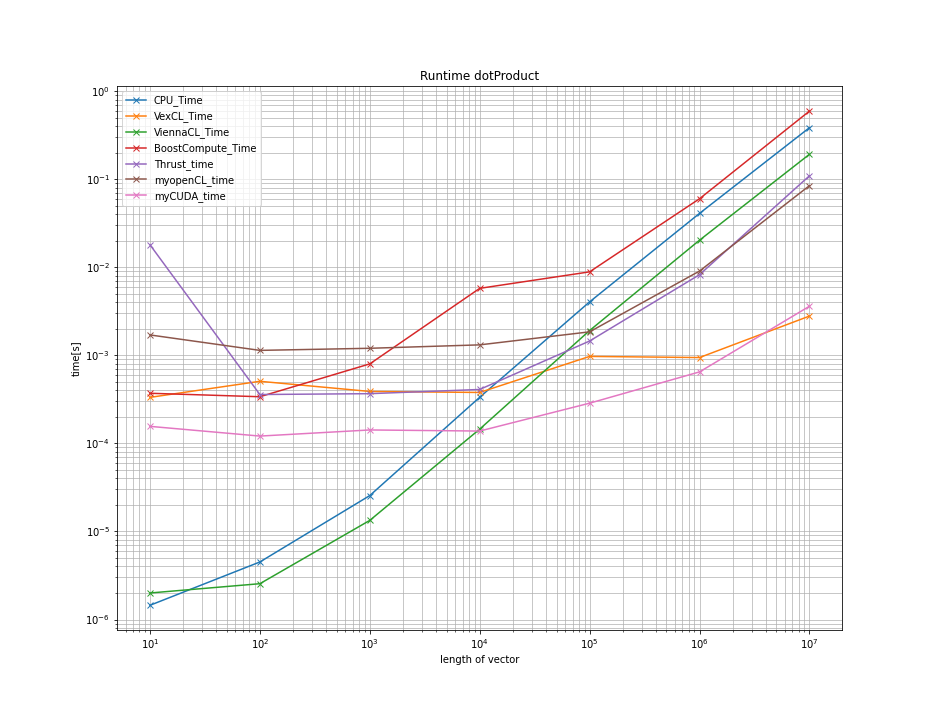
\includegraphics[width=\textwidth]{Bilder/Runtime_dotProduct}
	\end{minipage}
\end{center}
\noindent
I also included an implementation on the single CPU with two different kernels to have a reference more.\\
The winner of the benchmark is the VecCL library also interesting is that the time for that library VexCL does not grow as much as the other times.\\
The BoostCompute library has an out layer for the first point at a vector size of 10 but then the times behave like the VexCL library until a vector size of $10^5$. I expected that the CPU implementation is the slowest but the BoostCompute library is the slowest one.\\
MyCUDA implementation performs for the first 6 vector sizes better than all the others but for the last one VexCL wins.\\
MyopenCl implementation has the same shape as the myCUDA implementation with an offset $\rightarrow$ summation for the final dot-product result for the MyopenCl implementation done in the CPU part. 
\end{document}